\documentclass[pdftex, 10pt, a4paper]{report}

\usepackage[final]{pdfpages}
\newcommand{\HRule}{\rule{\linewidth}{0.5mm}}
\usepackage[toc,page]{appendix}
\usepackage{float}
\bibliography{Orientation.main.bib}
\usepackage{enumerate}
\usepackage{graphicx}
\usepackage[english]{babel}
\usepackage{footnote}
\usepackage{fancyhdr}
\usepackage{tabularx}
\usepackage{verbatim}
\usepackage{url}
\urlstyle{same}
%set to which level the toc goes, 1 = up to section, 2 includes subsection, etc
\setcounter{tocdepth}{1} 

\begin{document}

\pagestyle{fancy}
\fancyhead{}
\fancyhead[LE, LO] {\today}
\fancyhead[CE, CO] {Final Report}
\fancyhead[RE, RO] {version 1}

\begin{titlepage}

\begin{center}


% Upper part of the page

\textsc{\Large Technische Universiteit Delft }\\[1.5cm]
\textsc{\large TI3800 Bachelorproject}\\[0.5cm]
\textsc{\normalsize A non-centralized approach to Video on Demand on mobile devices}\\[0.5cm]


% Title
\HRule \\[0.4cm]
{ \huge \bfseries Architectural Design}\\[0.4cm]

\HRule \\[1.5cm]

% Author and supervisor
\begin{minipage}{0.4\textwidth}
\begin{flushleft} \large
\emph{Authors:}\\
Martijn \textsc{Breet} \\ (1265458) \\ [0.1cm]
Jaap \textsc{van Touw} \\(1380753)\\ [0.1cm]
\end{flushleft}
\end{minipage}
\begin{minipage}{0.4\textwidth}
\begin{flushright} \large
\emph{Supervisor:} \\
Cor-Paul \textsc{Bezemer}
\end{flushright}
\end{minipage}
\vspace{30mm}
\begin{figure}[ht!]
\centering

\includegraphics[width=50mm]{TUDLogo.png}
\hspace{10mm}

\includegraphics[width=50mm]{pdslogo.png}
\label{overflow}
\end{figure}
\vfill

% Bottom of the page
{\large \today}

\end{center}

\end{titlepage}


\tableofcontents
\pagebreak

\begin{abstract}
In this report, the different tools that could play a role for the Mobile Video-on-Demand project are elucidated. The main research question is: \textit{``How can we make video-on-demand available for mobile devices using a non-centralized approach?''}. A number of sub questions are derived from the main research question which deal with the different aspects of the main question separately. Android will be used as mobile platform because it holds the greatest market share and the team is proficient in programming for this platform. A number of Video-on-Demand solutions are described. In the end, Tribler is chosen because it uses a non-centralized approach, is free of costs for the user, has a large amount of videos available in HD and shows no advertisements. Tribler is not yet available for Android so it will have to be ported by using a python for Android tool. A multimedia framework must also be in the prototype for the playback of videos, VLC for Android Beta is chosen due to its state of maturity, popularity, number of codecs and modularity. If VLC should not work when the team attempts to implement it, Stagefright will be used as multimedia framework. If Python for Android does not work, Tribler can not be used and a plug-in will be written for VLC to incorporate main functionality. 
\end{abstract}

\pagebreak

%only in final version \chapter*{Preface}
\addcontentsline{toc}{chapter}{Preface}
This document entails the work of a Computer Science Bachelor project executed at the Delft Technical University within the Parallel and Distributed Systems group. I would like to offer my gratitude to the following people: \\

\emph{Cor-Paul Bezemer}, for his expert supervision, guidance and input.\\

\emph{Johan Pouwelse}, for his positive support, input and visionary influence.\\

\emph{Jan-Willem van Velzen}, for his fortunate mistake, partnership and his tireless effort in making a good application.\\

\emph{Egbert Bouman}, for his sublime tip at a most fortunate time.\\
\pagebreak

In this chapter the proposed prototype will be separated into different subsystems to give more insight into how to build the system. First the different subsystems will be elucidated, followed by an explanation on how the different subsystems interact with each other. The way the system stores data is clarified in section \ref{sec:perdata}. Different threads might try to alter the same part of data which causes a concurrency issue, when this would be possible and how the team will attempt to solve this is described in section \ref{sec:conc}. How information flows from subsystem to subsystem in different use cases can be seen in section \ref{sec:softctrl}. Another important part of the system is how it deals with starting and stopping as well as crashes, how this will be implemented is explained in the final section.									%part

\documentclass[pdftex, 10pt, a4paper]{report}

\newcommand{\HRule}{\rule{\linewidth}{0.5mm}}
\usepackage[style=numeric-comp]{biblatex}
\bibliography{planofaction.main.bib}
\usepackage{enumerate}
\usepackage{graphicx}
\usepackage[english]{babel}
\usepackage{fancyhdr}

\begin{document}

\pagestyle{fancy}
\fancyhead{}
\fancyhead[LE, LO] {\today}
\fancyhead[CE, CO] {Plan of Action}
\fancyhead[RE, RO] {version 1}

\begin{titlepage}

\begin{center}


% Upper part of the page

\textsc{\Large Technische Universiteit Delft }\\[1.5cm]
\textsc{\large TI3800 Bachelorproject}\\[0.5cm]
\textsc{\normalsize A non-centralized approach to Video on Demand on mobile devices}\\[0.5cm]


% Title
\HRule \\[0.4cm]
{ \huge \bfseries Architectural Design}\\[0.4cm]

\HRule \\[1.5cm]

% Author and supervisor
\begin{minipage}{0.4\textwidth}
\begin{flushleft} \large
\emph{Authors:}\\
Martijn \textsc{Breet} \\ (1265458) \\ [0.1cm]
Jaap \textsc{van Touw} \\(1380753)\\ [0.1cm]
\end{flushleft}
\end{minipage}
\begin{minipage}{0.4\textwidth}
\begin{flushright} \large
\emph{Supervisor:} \\
Cor-Paul \textsc{Bezemer}
\end{flushright}
\end{minipage}
\vspace{30mm}
\begin{figure}[ht!]
\centering

\includegraphics[width=50mm]{TUDLogo.png}
\hspace{10mm}

\includegraphics[width=50mm]{pdslogo.png}
\label{overflow}
\end{figure}
\vfill

% Bottom of the page
{\large \today}

\end{center}

\end{titlepage}


\tableofcontents

\pagebreak
\chapter*{Preface}
\addcontentsline{toc}{chapter}{Preface}
This document entails the work of a Computer Science Bachelor project executed at the Delft Technical University within the Parallel and Distributed Systems group. I would like to offer my gratitude to the following people: \\

\emph{Cor-Paul Bezemer}, for his expert supervision, guidance and input.\\

\emph{Johan Pouwelse}, for his positive support, input and visionary influence.\\

\emph{Jan-Willem van Velzen}, for his fortunate mistake, partnership and his tireless effort in making a good application.\\

\emph{Egbert Bouman}, for his sublime tip at a most fortunate time.\\							%preface
\pagebreak
\subsection*{Summary}
\addcontentsline{toc}{subsection}{Summary}
\thispagestyle{fancy}
							%summary

In this chapter the proposed prototype will be separated into different subsystems to give more insight into how to build the system. First the different subsystems will be elucidated, followed by an explanation on how the different subsystems interact with each other. The way the system stores data is clarified in section \ref{sec:perdata}. Different threads might try to alter the same part of data which causes a concurrency issue, when this would be possible and how the team will attempt to solve this is described in section \ref{sec:conc}. How information flows from subsystem to subsystem in different use cases can be seen in section \ref{sec:softctrl}. Another important part of the system is how it deals with starting and stopping as well as crashes, how this will be implemented is explained in the final section.				%chapter
\chapter{Project Assignment}
\thispagestyle{fancy}
In this chapter the proposed prototype will be separated into different subsystems to give more insight into how to build the system. First the different subsystems will be elucidated, followed by an explanation on how the different subsystems interact with each other. The way the system stores data is clarified in section \ref{sec:perdata}. Different threads might try to alter the same part of data which causes a concurrency issue, when this would be possible and how the team will attempt to solve this is described in section \ref{sec:conc}. How information flows from subsystem to subsystem in different use cases can be seen in section \ref{sec:softctrl}. Another important part of the system is how it deals with starting and stopping as well as crashes, how this will be implemented is explained in the final section.					%section
\section{Client}
The client is Dr. Ir. Johan Pouwelse, he is Assistant Professor at the Parallel and Distributed Systems Group of the Faculty of EEMCS, Delft University of Technology, and is also co-founder of Tribler. Moreover, he is Scientific director of several P2P research initiatives with a total budget of 26 Million Euro.						%section
\section{Stakeholders}
\textit{The Client:}\\
\\
\textbf{Dr. Ir. Johan Pouwelse}\\
J.A.Pouwelse@tudelft.nl\\
+31 (0)15 27 82539\\
Room: HB 07.290\\
Mekelweg 4\\
2628 CD Delft\\
\\
\textit{Project Supervisor:}\\
\\
\textbf{Cor-Paul Bezemer, MSc.}\\
C.Bezemer@tudelft.nl\\ 
+31 (0)15 27 82467\\
Mekelweg 4\\
2628 CD Delft\\
\\
\textit{Bachelor Project Coordinator:}\\
\\
\textbf{Dr. Martha A. Larson}\\
M.A.Larson@tudelft.nl\\
+31 (0)15 27 87357\\
Room: HB 11.040\\
Mekelweg 4\\
2628 CD Delft\\
				%section
\section{The Research question}
The project will be focused on answering the following main research question:\\
\\
\textit{``How can we make video-on-demand available for mobile devices using a non-centralized approach?''}

				%section
\section{Goal}
The goal of the project will be to create a prototype application for mobile devices, that allows users to enjoy video-on-demand through the Internet, using a non-centralized P2P network architecture. The application will allow users to search for a video, which will start playing after the user presses a play button. Additional seeking functionality will also be provided.
						%section
\section{Assignment Formulation}
In this project, a prototype of the P2P-based video-on-demand mobile application will be realized, that will allow users to search for videos on the Internet. Once the user has found a video to his or her liking, and issued a ‘play’ command, the application will play the video by means of streaming it through a P2P-based network. The application will also feature the possibility to seek to different parts of a video, by means of a slider, that can be adjusted by the user.
			%section
\section{Deliverables}
During and after the completion of the project, the following products will be delivered:\\
\begin{enumerate}
\item Orientation Report. 
\item Requirements Analysis Document
\item Architectural Design Document
\item Technical Design Document
\item Test- and Implementation Plan
\item Implementation (the prototype)
\item Source code evaluation by SIG\footnote{http://www.sig.eu}
\item Final report 
\end{enumerate}
The deliverables above are further defined in section 3.3.				%section
\section{Requirements and limitations}
The final product will offer the features that are described in section 2.6 and should be considered a ``proof of concept''. The prototype will offer video-on-demand, including built-in search functionality. The development of the prototype will be targeted to the Android platform. 
\section{Conditions}
The project members listed under section 4.2 will deliver the products listed in section 2.7 within a period of 11 weeks, starting from the 8th of july till the 20th of september 2013.\\
\\
The client will facilitate the project members in delivery of the deliverables by supplying them with all the resources needed for the development of these deliverables, such as (mobile) testing devices, required office space, etc.\\
\\
The project members will have weekly meetings with the Supervisor (see section 2.3) to discuss the status and progression of the project, as well as to receive feedback on completed work. These weekly meetings are also part of the development methodology which will be elucidated in section 3.2.		%section
%\section{Background and cause of assignment}
Distribution of radio and television programs, movies, music, ringtones, games, and various data applications to the general public is possible today via a variety of dedicated networks and special end user terminals. As broadband Internet becomes ubiquitous in both desktop and mobile device environments, all content distribution services will be combined and conveyed to the general public via a common pipeline, the Internet. Today several technologies are used for the media distribution across the Internet: unicast, IP multicast, content distribution networks, and most recently Peer-to-Peer. P2P is considered by many as an efficient, reliable, and low cost mechanism for distributing any media file or live stream, and it is used extensively. Much of the current research activities in P2P within the PDS group are centered around Tribler\footnote{http://www.tribler.org}. Tribler is an application that enables its users to find, enjoy and share content through a P2P network. Tribler builds on BitTorrent\footnote{http://www.bittorrent.com} and is currently only available on desktop environments. Currently mobile internet traffic continues to consistently gain on desktop traffic in terms of volume\footnote{http://gs.statcounter.com/mobile\_vs\_desktop\-ww\-monthly\-200812\-201306} and mobile traffic is estimated to surpass traffic from wired devices in 2017\footnote{http://www.cisco.com/en/US/solutions/collateral/ns341/ns525/ns537/ns705/ns827/VNI\_Hyperconnectivity\_WP.pdf}. In response to this growth and to meet the increasing demands of the market, the development of a mobile version of Tribler would be of great value. 
						%section		%chapter
\chapter{Approach}
\thispagestyle{fancy}
In this chapter the proposed prototype will be separated into different subsystems to give more insight into how to build the system. First the different subsystems will be elucidated, followed by an explanation on how the different subsystems interact with each other. The way the system stores data is clarified in section \ref{sec:perdata}. Different threads might try to alter the same part of data which causes a concurrency issue, when this would be possible and how the team will attempt to solve this is described in section \ref{sec:conc}. How information flows from subsystem to subsystem in different use cases can be seen in section \ref{sec:softctrl}. Another important part of the system is how it deals with starting and stopping as well as crashes, how this will be implemented is explained in the final section.						%section
\section{Orientation Phase}
In this phase, the research question is further crystallized into subquestions, which will create a better understanding of the problem as well its scope. After this is clarified, research will be conducted, by exploring existing (partial) solutions that can contribute towards a general solution for the problem. The findings of this research will be stated in the Orientation Report.

						%section
\section{Design Phase}
As a first step in the design phase, both functional-, nonfunctional requirements and constraints for the prototype will be elicited. From these requirements, usecases will be derived that convey how the system should interact with the user. Based on these requirements and use cases, an architectural design document will be created, consisting of a description of the proposed software architecture including subsystem decomposition, persistent data management, global resource handling, concurrency, software control and boundary conditions. Next, a detailed description of the packages, class diagram and a specification of the classes and methods is given in the Technical Design Document. Finally, a Test- and Implementation Plan is created that describes how the different features of the prototype are tested and implemented.


						%section
\section{Implementation Phase}
\label{sec:sig}
Building the application is the main part of the project and consists of implementing the different components that were derived in the Design Phase. The source code of the prototype will be sent to the SIG for a thorough review on the 5th of September. The feedback provided by the SIG will be used to improve the code during the implementation phase.					%section
\section{Release Phase}
In this final stage of the project, all the documents that were created during the previous phases of the project will be bundled into one final report. This will include a general conclusion and evaluation. After handing in the Final Report to the stakeholders, the source code of the prototype is sent to the SIG one more time for a final evaluation. The finished prototype will then be presented to the client, bachelor coordinator and supervisor. 						%section
\section{Methodology}
\label{sec:meth}
\subsection{Scrum}
During the project several methods will be put into practice. One of these methods, namely Scrum\footnote{http://www.scrum.org}, will be used in all phases starting from the design phase. Scrum is an iterative and incremental Agile method. Scrum uses sprints in which the team goes through the process of adding functionality to the software, always maintaining a working version of the prototype. Given the relatively small timespan of the project, sprints of one week are chosen to ensure progress is measured frequently. Traditionally, the Scrum method defines a number of roles assigning different responsibilities to each of the team members. Since the team for this project solely consists of two persons, no specific roles are assigned. At the start of each sprint, a meeting; called a sprint planning, will be held. These meetings will be attended by the team members, as well as the supervisor. In this manner, the supervisor gets a better insight into what progress is made and is able to provide more meaningful feedback on the previous and upcoming tasks. In the sprint planning the following is discussed:
\begin{itemize}
\item[-]Which tasks have been completed during the last sprint.
\item[-]Encountered impediments, if any.
\item[-]Decide on which tasks have to be done in the upcoming sprint.
\item[-]Determine the time it will take to complete the tasks and assign these to the team members.
\end{itemize}
The daily scrum meetings, also known as `standups', will only be attended by the team itself. During these meetings, the team will briefly discuss what each person did on the day before, what each person is going to do and if there are any impediments that need to be overcome. Furthermore, bi-weekly demo sessions will be held with the client, to keep the client informed on the progression that is made.
\subsection{MoSCoW}
\label{sec:moscow}
The MoSCoW method was first developed by by Clegg et al.\cite{moscow}, and it has become a standard in prioritizing a list of requirements. The following categories are defined:
\begin{itemize}
\item[-] Must have: requirements that must be satisfied in the final solution for the solution to be considered a success.
\item[-] Should have: high-priority requirements that should be included in the solution if possible.
\item[-] Could have: requirements which are considered desirable but not necessary.
\item[-] Would have: requirements that will not be implemented in a given release, but may be considered for the future.
\end{itemize}
The MoSCoW method will be used to prioritize the elicited requirements in the Requirements Analysis Document.
\subsection{Acceptance Testing}
\label{sec:acc_test}
Acceptance testing means that the team will see if the software in the current state meets the requirements by manually testing the functionality.						%section
\section{Planning}
A Gantt chart of the project planning can be found in Appendix A. The chart is complemented with a timeline, for a quick overview.
							%section					%chapter

\iffalse	
In this chapter the proposed prototype will be separated into different subsystems to give more insight into how to build the system. First the different subsystems will be elucidated, followed by an explanation on how the different subsystems interact with each other. The way the system stores data is clarified in section \ref{sec:perdata}. Different threads might try to alter the same part of data which causes a concurrency issue, when this would be possible and how the team will attempt to solve this is described in section \ref{sec:conc}. How information flows from subsystem to subsystem in different use cases can be seen in section \ref{sec:softctrl}. Another important part of the system is how it deals with starting and stopping as well as crashes, how this will be implemented is explained in the final section.						%chapter
\section{Goal of the proposed architecture}
					%section
\pagebreak
\fi

\end{document}
				%part
\part{Orientation}
\chapter{Introduction}
\thispagestyle{fancy}
In this chapter the proposed prototype will be separated into different subsystems to give more insight into how to build the system. First the different subsystems will be elucidated, followed by an explanation on how the different subsystems interact with each other. The way the system stores data is clarified in section \ref{sec:perdata}. Different threads might try to alter the same part of data which causes a concurrency issue, when this would be possible and how the team will attempt to solve this is described in section \ref{sec:conc}. How information flows from subsystem to subsystem in different use cases can be seen in section \ref{sec:softctrl}. Another important part of the system is how it deals with starting and stopping as well as crashes, how this will be implemented is explained in the final section.				%section
\section{Motivation}				%section
\section{Problem Statement}
As the previous section hinted, the following problem exists:\\
\\
\textit{``How can we make video-on-demand available for mobile devices using a non-centralized approach?''}\\

This research question consists out of three main elements: VoD, mobile devices and a non-centralized approach. These are the topics of  the following sub questions.

\subsection{Sub questions}
VoD is the main feature that needs to be considered for implementation, some existing applications on mobile and non-mobile devices (desktops for example) might already exist. Research in to this matter is crucial, so no redundant or useless work is done. This raises the following question:

\begin{enumerate}
	\item\textit{``Which solutions exist for VoD on (non-)mobile devices''}\\
	
	If no solutions exist for mobile devices, maybe there are solutions for non-mobile devices which can be ported to those mobile devices. This led to the following sub question:\\

		\begin{enumerate}
			\item\textit{``How can a port of an existing non-mobile solution be made to mobile devices?''}\\
			
			Important to realize is, that a port of a solution might not have full functionality because of hardware issues or other incompatibilities. Therefore research has to be done into the following:\\
			
			\item\textit{``What are the limitations of such a ported solution to mobile devices?''}\\
		\end{enumerate}

	Interesting to see is which of these solutions, ported or otherwise, use a non-centralized approach. Non-centralization is key to getting a low-cost, highly reliable and community driven solution. The following sub question pertains to this matter: \\

	\item\textit{``Which solutions for VoD use a non-centralized approach?''}\\

	There are an abundant number of different mobile devices, ranging from different sizes and processors to platforms. Each different platform, such Apple's iOS, Android and Windows phone, has its advantages and disadvantages. These pros and cons have to be researched in order to see which platforms are best suitable for which solutions. To conduct research in this topic, the following sub question was deduced:\\

	\item\textit{``Which mobile platforms are best suited to implement VoD in a non-centralized approach?''}\\
	
	Videos are encoded to save space and bandwidth once transmitted. To decode these videos, decoding software has to be used. Decoding software has to be included or linked to in order to play the video, research into this matter will be led by the following sub question:\\

	\item\textit{``What solutions exist for video decoding on the chosen platform?"}\\
\end{enumerate}

Research in the solution to sub question one will be conducted in chapter \ref{sec:vod}. In this same chapter, the non-centralization aspect as well as how a port can be made to mobile devices are described. The limitations of these ports are also described in this section. The different mobile platforms are elucidated in chapter \ref{sec:mos}. Video decoding is described in chapter \ref{sec:videc}. Finally an analysis of the risks involved is included in chapter \ref{sec:ra}, describing what to do when a situation arises that compromises a solution or part of it.			%section					%chapter
\chapter{Introduction}
\thispagestyle{fancy}
In this chapter the proposed prototype will be separated into different subsystems to give more insight into how to build the system. First the different subsystems will be elucidated, followed by an explanation on how the different subsystems interact with each other. The way the system stores data is clarified in section \ref{sec:perdata}. Different threads might try to alter the same part of data which causes a concurrency issue, when this would be possible and how the team will attempt to solve this is described in section \ref{sec:conc}. How information flows from subsystem to subsystem in different use cases can be seen in section \ref{sec:softctrl}. Another important part of the system is how it deals with starting and stopping as well as crashes, how this will be implemented is explained in the final section.				%section
\section{Motivation}				%section
\section{Problem Statement}
As the previous section hinted, the following problem exists:\\
\\
\textit{``How can we make video-on-demand available for mobile devices using a non-centralized approach?''}\\

This research question consists out of three main elements: VoD, mobile devices and a non-centralized approach. These are the topics of  the following sub questions.

\subsection{Sub questions}
VoD is the main feature that needs to be considered for implementation, some existing applications on mobile and non-mobile devices (desktops for example) might already exist. Research in to this matter is crucial, so no redundant or useless work is done. This raises the following question:

\begin{enumerate}
	\item\textit{``Which solutions exist for VoD on (non-)mobile devices''}\\
	
	If no solutions exist for mobile devices, maybe there are solutions for non-mobile devices which can be ported to those mobile devices. This led to the following sub question:\\

		\begin{enumerate}
			\item\textit{``How can a port of an existing non-mobile solution be made to mobile devices?''}\\
			
			Important to realize is, that a port of a solution might not have full functionality because of hardware issues or other incompatibilities. Therefore research has to be done into the following:\\
			
			\item\textit{``What are the limitations of such a ported solution to mobile devices?''}\\
		\end{enumerate}

	Interesting to see is which of these solutions, ported or otherwise, use a non-centralized approach. Non-centralization is key to getting a low-cost, highly reliable and community driven solution. The following sub question pertains to this matter: \\

	\item\textit{``Which solutions for VoD use a non-centralized approach?''}\\

	There are an abundant number of different mobile devices, ranging from different sizes and processors to platforms. Each different platform, such Apple's iOS, Android and Windows phone, has its advantages and disadvantages. These pros and cons have to be researched in order to see which platforms are best suitable for which solutions. To conduct research in this topic, the following sub question was deduced:\\

	\item\textit{``Which mobile platforms are best suited to implement VoD in a non-centralized approach?''}\\
	
	Videos are encoded to save space and bandwidth once transmitted. To decode these videos, decoding software has to be used. Decoding software has to be included or linked to in order to play the video, research into this matter will be led by the following sub question:\\

	\item\textit{``What solutions exist for video decoding on the chosen platform?"}\\
\end{enumerate}

Research in the solution to sub question one will be conducted in chapter \ref{sec:vod}. In this same chapter, the non-centralization aspect as well as how a port can be made to mobile devices are described. The limitations of these ports are also described in this section. The different mobile platforms are elucidated in chapter \ref{sec:mos}. Video decoding is described in chapter \ref{sec:videc}. Finally an analysis of the risks involved is included in chapter \ref{sec:ra}, describing what to do when a situation arises that compromises a solution or part of it.			%section				%chapter
\chapter{Introduction}
\thispagestyle{fancy}
In this chapter the proposed prototype will be separated into different subsystems to give more insight into how to build the system. First the different subsystems will be elucidated, followed by an explanation on how the different subsystems interact with each other. The way the system stores data is clarified in section \ref{sec:perdata}. Different threads might try to alter the same part of data which causes a concurrency issue, when this would be possible and how the team will attempt to solve this is described in section \ref{sec:conc}. How information flows from subsystem to subsystem in different use cases can be seen in section \ref{sec:softctrl}. Another important part of the system is how it deals with starting and stopping as well as crashes, how this will be implemented is explained in the final section.				%section
\section{Motivation}				%section
\section{Problem Statement}
As the previous section hinted, the following problem exists:\\
\\
\textit{``How can we make video-on-demand available for mobile devices using a non-centralized approach?''}\\

This research question consists out of three main elements: VoD, mobile devices and a non-centralized approach. These are the topics of  the following sub questions.

\subsection{Sub questions}
VoD is the main feature that needs to be considered for implementation, some existing applications on mobile and non-mobile devices (desktops for example) might already exist. Research in to this matter is crucial, so no redundant or useless work is done. This raises the following question:

\begin{enumerate}
	\item\textit{``Which solutions exist for VoD on (non-)mobile devices''}\\
	
	If no solutions exist for mobile devices, maybe there are solutions for non-mobile devices which can be ported to those mobile devices. This led to the following sub question:\\

		\begin{enumerate}
			\item\textit{``How can a port of an existing non-mobile solution be made to mobile devices?''}\\
			
			Important to realize is, that a port of a solution might not have full functionality because of hardware issues or other incompatibilities. Therefore research has to be done into the following:\\
			
			\item\textit{``What are the limitations of such a ported solution to mobile devices?''}\\
		\end{enumerate}

	Interesting to see is which of these solutions, ported or otherwise, use a non-centralized approach. Non-centralization is key to getting a low-cost, highly reliable and community driven solution. The following sub question pertains to this matter: \\

	\item\textit{``Which solutions for VoD use a non-centralized approach?''}\\

	There are an abundant number of different mobile devices, ranging from different sizes and processors to platforms. Each different platform, such Apple's iOS, Android and Windows phone, has its advantages and disadvantages. These pros and cons have to be researched in order to see which platforms are best suitable for which solutions. To conduct research in this topic, the following sub question was deduced:\\

	\item\textit{``Which mobile platforms are best suited to implement VoD in a non-centralized approach?''}\\
	
	Videos are encoded to save space and bandwidth once transmitted. To decode these videos, decoding software has to be used. Decoding software has to be included or linked to in order to play the video, research into this matter will be led by the following sub question:\\

	\item\textit{``What solutions exist for video decoding on the chosen platform?"}\\
\end{enumerate}

Research in the solution to sub question one will be conducted in chapter \ref{sec:vod}. In this same chapter, the non-centralization aspect as well as how a port can be made to mobile devices are described. The limitations of these ports are also described in this section. The different mobile platforms are elucidated in chapter \ref{sec:mos}. Video decoding is described in chapter \ref{sec:videc}. Finally an analysis of the risks involved is included in chapter \ref{sec:ra}, describing what to do when a situation arises that compromises a solution or part of it.			%section						%chapter 
\chapter{Introduction}
\thispagestyle{fancy}
In this chapter the proposed prototype will be separated into different subsystems to give more insight into how to build the system. First the different subsystems will be elucidated, followed by an explanation on how the different subsystems interact with each other. The way the system stores data is clarified in section \ref{sec:perdata}. Different threads might try to alter the same part of data which causes a concurrency issue, when this would be possible and how the team will attempt to solve this is described in section \ref{sec:conc}. How information flows from subsystem to subsystem in different use cases can be seen in section \ref{sec:softctrl}. Another important part of the system is how it deals with starting and stopping as well as crashes, how this will be implemented is explained in the final section.				%section
\section{Motivation}				%section
\section{Problem Statement}
As the previous section hinted, the following problem exists:\\
\\
\textit{``How can we make video-on-demand available for mobile devices using a non-centralized approach?''}\\

This research question consists out of three main elements: VoD, mobile devices and a non-centralized approach. These are the topics of  the following sub questions.

\subsection{Sub questions}
VoD is the main feature that needs to be considered for implementation, some existing applications on mobile and non-mobile devices (desktops for example) might already exist. Research in to this matter is crucial, so no redundant or useless work is done. This raises the following question:

\begin{enumerate}
	\item\textit{``Which solutions exist for VoD on (non-)mobile devices''}\\
	
	If no solutions exist for mobile devices, maybe there are solutions for non-mobile devices which can be ported to those mobile devices. This led to the following sub question:\\

		\begin{enumerate}
			\item\textit{``How can a port of an existing non-mobile solution be made to mobile devices?''}\\
			
			Important to realize is, that a port of a solution might not have full functionality because of hardware issues or other incompatibilities. Therefore research has to be done into the following:\\
			
			\item\textit{``What are the limitations of such a ported solution to mobile devices?''}\\
		\end{enumerate}

	Interesting to see is which of these solutions, ported or otherwise, use a non-centralized approach. Non-centralization is key to getting a low-cost, highly reliable and community driven solution. The following sub question pertains to this matter: \\

	\item\textit{``Which solutions for VoD use a non-centralized approach?''}\\

	There are an abundant number of different mobile devices, ranging from different sizes and processors to platforms. Each different platform, such Apple's iOS, Android and Windows phone, has its advantages and disadvantages. These pros and cons have to be researched in order to see which platforms are best suitable for which solutions. To conduct research in this topic, the following sub question was deduced:\\

	\item\textit{``Which mobile platforms are best suited to implement VoD in a non-centralized approach?''}\\
	
	Videos are encoded to save space and bandwidth once transmitted. To decode these videos, decoding software has to be used. Decoding software has to be included or linked to in order to play the video, research into this matter will be led by the following sub question:\\

	\item\textit{``What solutions exist for video decoding on the chosen platform?"}\\
\end{enumerate}

Research in the solution to sub question one will be conducted in chapter \ref{sec:vod}. In this same chapter, the non-centralization aspect as well as how a port can be made to mobile devices are described. The limitations of these ports are also described in this section. The different mobile platforms are elucidated in chapter \ref{sec:mos}. Video decoding is described in chapter \ref{sec:videc}. Finally an analysis of the risks involved is included in chapter \ref{sec:ra}, describing what to do when a situation arises that compromises a solution or part of it.			%section					%chapter
\chapter{Introduction}
\thispagestyle{fancy}
In this chapter the proposed prototype will be separated into different subsystems to give more insight into how to build the system. First the different subsystems will be elucidated, followed by an explanation on how the different subsystems interact with each other. The way the system stores data is clarified in section \ref{sec:perdata}. Different threads might try to alter the same part of data which causes a concurrency issue, when this would be possible and how the team will attempt to solve this is described in section \ref{sec:conc}. How information flows from subsystem to subsystem in different use cases can be seen in section \ref{sec:softctrl}. Another important part of the system is how it deals with starting and stopping as well as crashes, how this will be implemented is explained in the final section.				%section
\section{Motivation}				%section
\section{Problem Statement}
As the previous section hinted, the following problem exists:\\
\\
\textit{``How can we make video-on-demand available for mobile devices using a non-centralized approach?''}\\

This research question consists out of three main elements: VoD, mobile devices and a non-centralized approach. These are the topics of  the following sub questions.

\subsection{Sub questions}
VoD is the main feature that needs to be considered for implementation, some existing applications on mobile and non-mobile devices (desktops for example) might already exist. Research in to this matter is crucial, so no redundant or useless work is done. This raises the following question:

\begin{enumerate}
	\item\textit{``Which solutions exist for VoD on (non-)mobile devices''}\\
	
	If no solutions exist for mobile devices, maybe there are solutions for non-mobile devices which can be ported to those mobile devices. This led to the following sub question:\\

		\begin{enumerate}
			\item\textit{``How can a port of an existing non-mobile solution be made to mobile devices?''}\\
			
			Important to realize is, that a port of a solution might not have full functionality because of hardware issues or other incompatibilities. Therefore research has to be done into the following:\\
			
			\item\textit{``What are the limitations of such a ported solution to mobile devices?''}\\
		\end{enumerate}

	Interesting to see is which of these solutions, ported or otherwise, use a non-centralized approach. Non-centralization is key to getting a low-cost, highly reliable and community driven solution. The following sub question pertains to this matter: \\

	\item\textit{``Which solutions for VoD use a non-centralized approach?''}\\

	There are an abundant number of different mobile devices, ranging from different sizes and processors to platforms. Each different platform, such Apple's iOS, Android and Windows phone, has its advantages and disadvantages. These pros and cons have to be researched in order to see which platforms are best suitable for which solutions. To conduct research in this topic, the following sub question was deduced:\\

	\item\textit{``Which mobile platforms are best suited to implement VoD in a non-centralized approach?''}\\
	
	Videos are encoded to save space and bandwidth once transmitted. To decode these videos, decoding software has to be used. Decoding software has to be included or linked to in order to play the video, research into this matter will be led by the following sub question:\\

	\item\textit{``What solutions exist for video decoding on the chosen platform?"}\\
\end{enumerate}

Research in the solution to sub question one will be conducted in chapter \ref{sec:vod}. In this same chapter, the non-centralization aspect as well as how a port can be made to mobile devices are described. The limitations of these ports are also described in this section. The different mobile platforms are elucidated in chapter \ref{sec:mos}. Video decoding is described in chapter \ref{sec:videc}. Finally an analysis of the risks involved is included in chapter \ref{sec:ra}, describing what to do when a situation arises that compromises a solution or part of it.			%section					%chapter
			%part
\chapter{Introduction}
\thispagestyle{fancy}
In this chapter the proposed prototype will be separated into different subsystems to give more insight into how to build the system. First the different subsystems will be elucidated, followed by an explanation on how the different subsystems interact with each other. The way the system stores data is clarified in section \ref{sec:perdata}. Different threads might try to alter the same part of data which causes a concurrency issue, when this would be possible and how the team will attempt to solve this is described in section \ref{sec:conc}. How information flows from subsystem to subsystem in different use cases can be seen in section \ref{sec:softctrl}. Another important part of the system is how it deals with starting and stopping as well as crashes, how this will be implemented is explained in the final section.				%section
\section{Motivation}				%section
\section{Problem Statement}
As the previous section hinted, the following problem exists:\\
\\
\textit{``How can we make video-on-demand available for mobile devices using a non-centralized approach?''}\\

This research question consists out of three main elements: VoD, mobile devices and a non-centralized approach. These are the topics of  the following sub questions.

\subsection{Sub questions}
VoD is the main feature that needs to be considered for implementation, some existing applications on mobile and non-mobile devices (desktops for example) might already exist. Research in to this matter is crucial, so no redundant or useless work is done. This raises the following question:

\begin{enumerate}
	\item\textit{``Which solutions exist for VoD on (non-)mobile devices''}\\
	
	If no solutions exist for mobile devices, maybe there are solutions for non-mobile devices which can be ported to those mobile devices. This led to the following sub question:\\

		\begin{enumerate}
			\item\textit{``How can a port of an existing non-mobile solution be made to mobile devices?''}\\
			
			Important to realize is, that a port of a solution might not have full functionality because of hardware issues or other incompatibilities. Therefore research has to be done into the following:\\
			
			\item\textit{``What are the limitations of such a ported solution to mobile devices?''}\\
		\end{enumerate}

	Interesting to see is which of these solutions, ported or otherwise, use a non-centralized approach. Non-centralization is key to getting a low-cost, highly reliable and community driven solution. The following sub question pertains to this matter: \\

	\item\textit{``Which solutions for VoD use a non-centralized approach?''}\\

	There are an abundant number of different mobile devices, ranging from different sizes and processors to platforms. Each different platform, such Apple's iOS, Android and Windows phone, has its advantages and disadvantages. These pros and cons have to be researched in order to see which platforms are best suitable for which solutions. To conduct research in this topic, the following sub question was deduced:\\

	\item\textit{``Which mobile platforms are best suited to implement VoD in a non-centralized approach?''}\\
	
	Videos are encoded to save space and bandwidth once transmitted. To decode these videos, decoding software has to be used. Decoding software has to be included or linked to in order to play the video, research into this matter will be led by the following sub question:\\

	\item\textit{``What solutions exist for video decoding on the chosen platform?"}\\
\end{enumerate}

Research in the solution to sub question one will be conducted in chapter \ref{sec:vod}. In this same chapter, the non-centralization aspect as well as how a port can be made to mobile devices are described. The limitations of these ports are also described in this section. The different mobile platforms are elucidated in chapter \ref{sec:mos}. Video decoding is described in chapter \ref{sec:videc}. Finally an analysis of the risks involved is included in chapter \ref{sec:ra}, describing what to do when a situation arises that compromises a solution or part of it.			%section					%part
\documentclass[pdftex, 12pt, a4paper]{report}

\newcommand{\HRule}{\rule{\linewidth}{0.5mm}}
\usepackage{enumerate}
\usepackage{enumitem}
\usepackage{graphicx}
\usepackage[english]{babel}
\usepackage{fancyhdr}
\usepackage{supertabular}

\begin{document}

\pagestyle{fancy}
\fancyhead{}
\fancyhead[LE, LO] {\today}
\fancyhead[CE, CO] {Test and Implementationplan}
\fancyhead[RE, RO] {version 2}

\begin{titlepage}

\begin{center}


% Upper part of the page

\textsc{\Large Technische Universiteit Delft }\\[1.5cm]
\textsc{\large TI3800 Bachelorproject}\\[0.5cm]
\textsc{\normalsize A non-centralized approach to Video on Demand on mobile devices}\\[0.5cm]


% Title
\HRule \\[0.4cm]
{ \huge \bfseries Architectural Design}\\[0.4cm]

\HRule \\[1.5cm]

% Author and supervisor
\begin{minipage}{0.4\textwidth}
\begin{flushleft} \large
\emph{Authors:}\\
Martijn \textsc{Breet} \\ (1265458) \\ [0.1cm]
Jaap \textsc{van Touw} \\(1380753)\\ [0.1cm]
\end{flushleft}
\end{minipage}
\begin{minipage}{0.4\textwidth}
\begin{flushright} \large
\emph{Supervisor:} \\
Cor-Paul \textsc{Bezemer}
\end{flushright}
\end{minipage}
\vspace{30mm}
\begin{figure}[ht!]
\centering

\includegraphics[width=50mm]{TUDLogo.png}
\hspace{10mm}

\includegraphics[width=50mm]{pdslogo.png}
\label{overflow}
\end{figure}
\vfill

% Bottom of the page
{\large \today}

\end{center}

\end{titlepage}


\pagebreak

\tableofcontents

\pagebreak

In this chapter the proposed prototype will be separated into different subsystems to give more insight into how to build the system. First the different subsystems will be elucidated, followed by an explanation on how the different subsystems interact with each other. The way the system stores data is clarified in section \ref{sec:perdata}. Different threads might try to alter the same part of data which causes a concurrency issue, when this would be possible and how the team will attempt to solve this is described in section \ref{sec:conc}. How information flows from subsystem to subsystem in different use cases can be seen in section \ref{sec:softctrl}. Another important part of the system is how it deals with starting and stopping as well as crashes, how this will be implemented is explained in the final section.		%chapter
\chapter{Testing}
\label{sec:test}
This chapter provides insight into how testing will be done in this project. The first section will explain how unit testing will be incorporated  in the project, which is followed by a section about acceptance testing.

\section{Unit Testing}
Every function or method can be modeled as a black box, where the black box processes the input and generates the output. To test if the correct output is generated, unit testing is used. Within a unit test the tester can define the input and what the expected output is, then the unit test runs and tests if the function's output is the same as the expected output. If not it will warn the tester that the test failed so the function can be changed to behave correctly. 
In this project the team will test all methods that have adequate logic in them. For example, getters and setters will not be tested. Methods from third-party software like Tribler and VLC will also not be tested separately. 

\section{Acceptance testing}
Acceptance testing means that the team will see if the software in the current state meets the requirements by manually testing the functionality. In the different sprints, functionality will be added to the prototype. Acceptance testing will be done in between the sprints to ensure that the prototype meets the requirements set to be implemented for that sprint.			%chapter
\chapter{Implementation}
\thispagestyle{fancy}
\label{sec:impl}
In the Requirements Analysis, the requirements were prioritized according to the MoSCoW method. The priority in that document will be a guideline to plan the different stages of implementation. Every sprint planning, a number of functional requirements will be implemented as functionality to the prototype. For the explanation of the requirements, please see the Requirements Analysis. The following planning is subject to the risks involved, which are elucidated in the Orientation Phase and could therefore not be accurate later on in the project.

\section{Sprint planning one}
In sprint planning one, the aim will be to let a predetermined video, play on Android via VLC. This satisfies the requirement of playing a video. When this functions correctly, the requirements of pausing and seeking in a video are also satisfied because they depend on VLC. Acceptance testing will be used to test if this is indeed the case.
\section{Sprint planning two}
In this sprint planning the goal will be to incorporate the Tribler core in to the mix. Making the python-based program work on Android will be the challenge in this sprint planning. The Tribler core, which includes Libtorrent, should be capable of downloading a video on Android and together with the work done in sprint planning one, the prototype should now be able to download a predetermined video and let it play through the use of VLC. Testing will be done afterwards to check if the prototype meets the currently set requirements.
\section{Sprint planning three}
When the download algorithm is adapted for streaming, the prototype can stream the video directly to VLC instead of first downloading it. The prototype should have all the `must have' requirements now, to test if this is the case, acceptance testing is used.
\section{Sprint planning four}
Tribler has a search function which searches for videos to download in a non-centralized way. In this sprint planning the team will attempt to incorporate the search function so users can search for a video, click play and then the video will be streamed to their device. Again, acceptance testing will be used before the next sprint planning to check if the prototype is still in a fully working state.
\section{Sprint planning five}
The last sprint planning will be to incorporate the requirement to optionally download a video. A single click installer will also be provided to incorporate VLC and Tribler into one single .apk file (the install file format for Android). After this, the prototype will be subjected to acceptance testing to check if everything works as intended.		%chapter

\pagebreak

\end{document}
	%part

\chapter{Introduction}
\thispagestyle{fancy}
In this chapter the proposed prototype will be separated into different subsystems to give more insight into how to build the system. First the different subsystems will be elucidated, followed by an explanation on how the different subsystems interact with each other. The way the system stores data is clarified in section \ref{sec:perdata}. Different threads might try to alter the same part of data which causes a concurrency issue, when this would be possible and how the team will attempt to solve this is described in section \ref{sec:conc}. How information flows from subsystem to subsystem in different use cases can be seen in section \ref{sec:softctrl}. Another important part of the system is how it deals with starting and stopping as well as crashes, how this will be implemented is explained in the final section.				%section
\section{Motivation}				%section
\section{Problem Statement}
As the previous section hinted, the following problem exists:\\
\\
\textit{``How can we make video-on-demand available for mobile devices using a non-centralized approach?''}\\

This research question consists out of three main elements: VoD, mobile devices and a non-centralized approach. These are the topics of  the following sub questions.

\subsection{Sub questions}
VoD is the main feature that needs to be considered for implementation, some existing applications on mobile and non-mobile devices (desktops for example) might already exist. Research in to this matter is crucial, so no redundant or useless work is done. This raises the following question:

\begin{enumerate}
	\item\textit{``Which solutions exist for VoD on (non-)mobile devices''}\\
	
	If no solutions exist for mobile devices, maybe there are solutions for non-mobile devices which can be ported to those mobile devices. This led to the following sub question:\\

		\begin{enumerate}
			\item\textit{``How can a port of an existing non-mobile solution be made to mobile devices?''}\\
			
			Important to realize is, that a port of a solution might not have full functionality because of hardware issues or other incompatibilities. Therefore research has to be done into the following:\\
			
			\item\textit{``What are the limitations of such a ported solution to mobile devices?''}\\
		\end{enumerate}

	Interesting to see is which of these solutions, ported or otherwise, use a non-centralized approach. Non-centralization is key to getting a low-cost, highly reliable and community driven solution. The following sub question pertains to this matter: \\

	\item\textit{``Which solutions for VoD use a non-centralized approach?''}\\

	There are an abundant number of different mobile devices, ranging from different sizes and processors to platforms. Each different platform, such Apple's iOS, Android and Windows phone, has its advantages and disadvantages. These pros and cons have to be researched in order to see which platforms are best suitable for which solutions. To conduct research in this topic, the following sub question was deduced:\\

	\item\textit{``Which mobile platforms are best suited to implement VoD in a non-centralized approach?''}\\
	
	Videos are encoded to save space and bandwidth once transmitted. To decode these videos, decoding software has to be used. Decoding software has to be included or linked to in order to play the video, research into this matter will be led by the following sub question:\\

	\item\textit{``What solutions exist for video decoding on the chosen platform?"}\\
\end{enumerate}

Research in the solution to sub question one will be conducted in chapter \ref{sec:vod}. In this same chapter, the non-centralization aspect as well as how a port can be made to mobile devices are described. The limitations of these ports are also described in this section. The different mobile platforms are elucidated in chapter \ref{sec:mos}. Video decoding is described in chapter \ref{sec:videc}. Finally an analysis of the risks involved is included in chapter \ref{sec:ra}, describing what to do when a situation arises that compromises a solution or part of it.			%section							%part
\chapter{Introduction}
\thispagestyle{fancy}
In this chapter the proposed prototype will be separated into different subsystems to give more insight into how to build the system. First the different subsystems will be elucidated, followed by an explanation on how the different subsystems interact with each other. The way the system stores data is clarified in section \ref{sec:perdata}. Different threads might try to alter the same part of data which causes a concurrency issue, when this would be possible and how the team will attempt to solve this is described in section \ref{sec:conc}. How information flows from subsystem to subsystem in different use cases can be seen in section \ref{sec:softctrl}. Another important part of the system is how it deals with starting and stopping as well as crashes, how this will be implemented is explained in the final section.				%section
\section{Motivation}				%section
\section{Problem Statement}
As the previous section hinted, the following problem exists:\\
\\
\textit{``How can we make video-on-demand available for mobile devices using a non-centralized approach?''}\\

This research question consists out of three main elements: VoD, mobile devices and a non-centralized approach. These are the topics of  the following sub questions.

\subsection{Sub questions}
VoD is the main feature that needs to be considered for implementation, some existing applications on mobile and non-mobile devices (desktops for example) might already exist. Research in to this matter is crucial, so no redundant or useless work is done. This raises the following question:

\begin{enumerate}
	\item\textit{``Which solutions exist for VoD on (non-)mobile devices''}\\
	
	If no solutions exist for mobile devices, maybe there are solutions for non-mobile devices which can be ported to those mobile devices. This led to the following sub question:\\

		\begin{enumerate}
			\item\textit{``How can a port of an existing non-mobile solution be made to mobile devices?''}\\
			
			Important to realize is, that a port of a solution might not have full functionality because of hardware issues or other incompatibilities. Therefore research has to be done into the following:\\
			
			\item\textit{``What are the limitations of such a ported solution to mobile devices?''}\\
		\end{enumerate}

	Interesting to see is which of these solutions, ported or otherwise, use a non-centralized approach. Non-centralization is key to getting a low-cost, highly reliable and community driven solution. The following sub question pertains to this matter: \\

	\item\textit{``Which solutions for VoD use a non-centralized approach?''}\\

	There are an abundant number of different mobile devices, ranging from different sizes and processors to platforms. Each different platform, such Apple's iOS, Android and Windows phone, has its advantages and disadvantages. These pros and cons have to be researched in order to see which platforms are best suitable for which solutions. To conduct research in this topic, the following sub question was deduced:\\

	\item\textit{``Which mobile platforms are best suited to implement VoD in a non-centralized approach?''}\\
	
	Videos are encoded to save space and bandwidth once transmitted. To decode these videos, decoding software has to be used. Decoding software has to be included or linked to in order to play the video, research into this matter will be led by the following sub question:\\

	\item\textit{``What solutions exist for video decoding on the chosen platform?"}\\
\end{enumerate}

Research in the solution to sub question one will be conducted in chapter \ref{sec:vod}. In this same chapter, the non-centralization aspect as well as how a port can be made to mobile devices are described. The limitations of these ports are also described in this section. The different mobile platforms are elucidated in chapter \ref{sec:mos}. Video decoding is described in chapter \ref{sec:videc}. Finally an analysis of the risks involved is included in chapter \ref{sec:ra}, describing what to do when a situation arises that compromises a solution or part of it.			%section					%part

\begin{thebibliography}{9}

\bibitem{internet_study}
  	Hendrik Schulze, Klaus Mochalski,
  	\emph{Internet Study 2008/2009},
 	Ipoque, Germany,
  	2009.

\bibitem{moscow}
	Dai Clegg, Richard Barker,  
	\emph{Case Method Fast-Track: A RAD Approach}
	Addison-Wesley,
	2004.

\bibitem{libswift12}
  	 R. Petrocco, J. Pouwelse and D.H.J. Epema,
  	\emph{Performance Analysis of the Libswift P2P Streaming Protocol},
  	IEEE P2P, TU Delft,
  	2012.

\bibitem{tribler}
   	J.A. Pouwelse, P. Garbacki, J. Wang, A. Bakker, J. Yang, A. Iosup, D.H.J. Epema, M. Reinders, M. van Steen, H.J. Sips,
  	\emph{Tribler: A social-based Peer-to-Peer system},
  	TU Delft, Vrije Universiteit Amsterdam,
  	2006.

\bibitem{dispersy}
   	Niels Zeilemaker, Boudewijn Schoon, Johan Pouwelse,
  	\emph{Dispersy Bundle Synchronization},
  	TU Delft, Parallel and Distributed Systems,
  	January 2013.

\bibitem{compnet}
	Andrew S. Tanenbaum, David J. Wetherall,
 	\emph{Computer Networks},
	5th edition,
	Pearson Education,
	2010.

\end{thebibliography}
\begin{appendices}
\thispagestyle{fancy}
\chapter{Project Planning}					%generate chapter for each Appendix
%\section{Introduction}	%subsections not really needed in this Appendix
\begin{figure}[ht!]
\hspace*{-1in}
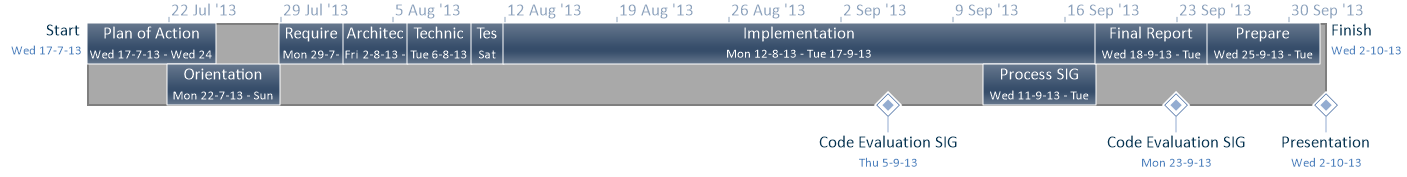
\includegraphics[width=170mm]{../../Planning/timeline.png}
\hspace*{-1in}
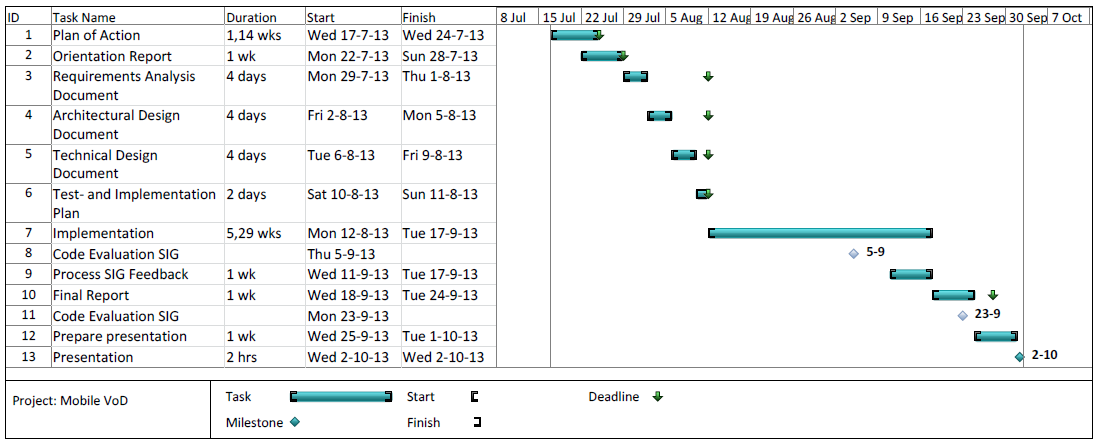
\includegraphics[width=170mm]{../../Planning/ProjectPlanning.png}
\end{figure}

					%content of the Appendix		%chapter
%input meeting minutes
\chapter{Build Instructions VLC}
\label{sec:app_vlc_build}
\paragraph{ENVIRONMENT} \mbox{}\\
install:
\begin{itemize}
\item Oracle JDK SE `latest' (tested on 7u25)
\item Android ADT bundle (follow instructions on the download site)
\item Android NDK R9 (including legacy toolchains)
\end{itemize}

\paragraph{SETUP}\mbox{}\\
Edit environment variables:
\\
sudo gedit /etc/environment\\
add ANDROID\_SDK=/home/user/android/android-sdk-linux\\
add ANDROID\_NDK=/home/user/android/android-ndk-r9\\
add ANDROID\_ABI=armeabi-v7a\\

Add to PATH environment variable:\\
/home/user/android/android-sdk-linux/platform-tools:/home/user/android/android-sdk-linux/tools\\
install the following tools: \\
apache-ant (or ant), autoconf, automake, autopoint,cmake, gawk (or nawk), gcc, g++, ia32-libs, build-essential, libtool, m4, patch, pkg-config, ragel, subversion, and up-to-date versions of those tools.\\
\\
On the command line:\\
sudo apt-get install ant autoconf automake autopoint cmake gawk gcc g++ ia32-libs build-essential libtool m4 patch pkg-config ragel subversion\\
\\
Get the source code:\\
git clone git://git.videolan.org/vlc-ports/android.git VLC\\

\paragraph{COMPILING PROCESS}\mbox{}\\
Go in to the folder VLC\\
gedit /compile.sh\\
Edit the mcpu flags for the appropriate target CPU (cortex-a15 for Nexus 10)\\
gedit /vlc-android/jni/Application.mk\\
Modify content into NDK\_TOOLCHAIN\_VERSION=4.8\\
sh compile.sh\\
\\
Compiling should be done, go to device installation instructions\\

\paragraph{COMPILING TROUBLESHOOT}\mbox{}\\
If the compiling stops unsuccessfully, run the following command: find \~/vlcsourcefolder/ -name ``udiv.asm"\\
Edit each file from the search results, and remove the spaces between the [ ] brackets, if any.\\
sh compile.sh (start the compilation again, it will now successfully continue and finish)\\

\paragraph{TARGET DEVICE INSTALLATION INSTRUCTIONS:}\mbox{}\\
cd /vlc-android/bin/ folder\\
Install the apk file with the 'adb install filename.apk' command\\

\paragraph{ECLIPSE}\mbox{}\\
You can load the project into eclipse(preferably from the ADT bundle) by importing android project from existing source. (new project-Android-Android project from existing code).\\
Guide the wizard to your vlc folder and load the four projects that the wizard found.\\
Be sure to set the dependencies in the VLC project correctly by right-clicking on that project, go to the Android tab, and setting the three other projects as libraries for VLC.\\
You can now run and debug VLC from the Eclipse environment.\\

\end{appendices}
\end{document}
